\documentclass[a4paper,12pt]{report}
\usepackage[utf8]{inputenc}
\usepackage[T1]{fontenc}
\usepackage[french]{babel}
\usepackage{amsmath}
\usepackage{amssymb}
\usepackage{graphicx}
\usepackage{float}
\usepackage{setspace}
\usepackage{hyperref}
\usepackage{listings}
\usepackage{color}
\usepackage{geometry}
\geometry{top=3cm, bottom=3cm, left=2.5cm, right=2.5cm}
\usepackage{fancyhdr}
\usepackage{array}
\usepackage{booktabs}
\usepackage{multirow}
\usepackage{eso-pic}
\usepackage{tabularx}
\usepackage{enumitem}
\usepackage{tcolorbox}
\tcbuselibrary{skins, breakable}
\usepackage{tikz}
\usetikzlibrary{shapes.geometric, arrows.meta, positioning}
\usepackage{pgfplots}
\pgfplotsset{compat=1.18}

\pagestyle{fancy}
\fancyhf{}
\fancyfoot[C]{\textbf{\thepage}}

% Couleurs
\definecolor{primary}{HTML}{1A237E}
\definecolor{accent}{HTML}{0288D1}
\definecolor{bbgreen}{HTML}{2E7D32}
\definecolor{pplred}{HTML}{C62828}
\definecolor{lightgray}{HTML}{F5F5F5}

% tcolorbox style
\tcbset{
  mybox/.style={
    enhanced, breakable,
    colback=lightgray,
    colframe=accent,
    fonttitle=\bfseries,
    boxrule=0.8pt,
    arc=4pt,
  }
}

% Configuration listings
\definecolor{codegreen}{rgb}{0,0.6,0}
\definecolor{codegray}{rgb}{0.5,0.5,0.5}
\definecolor{codepurple}{rgb}{0.58,0,0.82}
\definecolor{backcolour}{rgb}{0.95,0.95,0.92}
\lstdefinestyle{mystyle}{
    backgroundcolor=\color{backcolour},
    commentstyle=\color{codegreen},
    keywordstyle=\color{magenta},
    numberstyle=\tiny\color{codegray},
    stringstyle=\color{codepurple},
    basicstyle=\ttfamily\footnotesize,
    breakatwhitespace=false,
    breaklines=true,
    captionpos=b,
    keepspaces=true,
    numbers=left,
    numbersep=5pt,
    showspaces=false,
    showstringspaces=false,
    showtabs=false,
    tabsize=2
}
\lstset{style=mystyle}

\usepackage{tocloft}
\renewcommand{\contentsname}{\begin{center}\textbf{\huge Table des matières}\end{center}}
\renewcommand{\listfigurename}{\begin{center}\textbf{\huge Liste des figures}\end{center}}
\renewcommand{\listtablename}{\begin{center}\textbf{\huge Liste des tableaux}\end{center}}

\begin{document}

% ==========================================================
% PAGE DE GARDE
% ==========================================================
\begin{titlepage}
\centering
\pagestyle{empty}

\AddToShipoutPictureBG*{
    
\includegraphics[width=\paperwidth,height=\paperheight]{logos/background.png}
}

\vspace*{-0.8cm}
\makebox[\textwidth]{%
    
\includegraphics[height=4.2cm]{logos/ensias.png}
    \hfill
    
\includegraphics[height=4.2cm]{logos/um5logo.png}
}

\vspace{0.8cm}
\textsc{\large École Nationale Supérieure \\[0.2cm] d'Informatique et d'Analyse des Systèmes - Rabat}

\vspace{0.8cm}
\large Filière : Génie de la Data

\vspace{1.5cm}

\textcolor{black}{\rule{\textwidth}{2pt}}\\[0.5cm]
{\Huge \bfseries Basal-Bolus vs Reinforcement Learning : Contrôle automatique du dosage d'insuline pour les patients atteints de Diabète de Type 1\\[1cm]}
\textcolor{black}{\rule{\textwidth}{2pt}}\\[1cm]

\vspace{0.5cm}
\begin{flushleft}
\large
\begin{tabular}{@{} l @{\hspace{3.5cm}} l @{}}
\emph{Réalisé par :} & \emph{Encadrants :} \\[0.3cm]
Anass Bensmina      & Pr. Gasmini Manal \\
Moubarak Benaqqa    & Pr. Rachid Oulad Haj Thami \\
Karim Ait Salim & \\
\end{tabular}
\end{flushleft}




\vfill
{\large Année Universitaire : 2025/2026}

\end{titlepage}

% ── Table des matières ────────────────────────────────────────────────────────
\tableofcontents
\newpage

% ════════════════════════════════════════════════════════════════════════════
\chapter{Résumé}

Ce rapport présente une étude comparative entre un contrôleur \textbf{Basal-Bolus}, qui constitue la norme de soin clinique actuelle pour le traitement du Diabète de Type~1, et un agent d'\textbf{Apprentissage par Renforcement} (PPO, \textit{Proximal Policy Optimization}) pour la gestion automatique du dosage d'insuline chez des patients virtuels. Les expériences sont conduites dans le simulateur physiologique \textit{SimGlucose}, basé sur le modèle UVA/Padova approuvé par la FDA, sur une cohorte de 6 patients (3 adultes, 3 adolescents) et 50 épisodes de 24 heures par patient. Les performances sont mesurées à l'aide de métriques cliniques standardisées : \textit{Time-In-Range} (TIR), \textit{Time Below Range} (TBR), \textit{Time Above Range} (TAR), ainsi que les indices de risque LBGI et HBGI.

Les résultats révèlent une tension fondamentale entre les deux approches : le contrôleur Basal-Bolus obtient un TIR médian de \textbf{80.87\%} contre \textbf{74.81\%} pour l'agent PPO, mais au prix d'un taux d'échec de \textbf{82.3\%} (épisodes avec au moins une glycémie inférieure à 40 mg/dL), contre \textbf{0\%} pour l'agent PPO. Autrement dit, le Basal-Bolus offre un meilleur contrôle moyen mais induit régulièrement des hypoglycémies sévères potentiellement mortelles, tandis que l'agent appris par renforcement opère dans une enveloppe sûre, sans jamais atteindre les extrêmes dangereux.

\begin{tcolorbox}[mybox, title=Points clés]
\begin{itemize}[noitemsep]
  \item L'agent PPO apprend \emph{sans} recevoir d'annonce de repas, contrairement au contrôleur Basal-Bolus qui reçoit le contenu glucidique des repas en avance.
  \item Le protocole expérimental couvre 6 profils physiologiques distincts et 50 graines aléatoires par patient.
  \item La comparaison statistique repose sur le test de Mann-Whitney U avec taille d'effet (Cohen's~$r$).
  \item Le cadre méthodologique reproduit celui du papier G2P2C (Hettiarachchi et al., 2024).
\end{itemize}
\end{tcolorbox}

\newpage

% ════════════════════════════════════════════════════════════════════════════
\chapter{Introduction}

\section{Contexte médical}

Le Diabète de Type~1 est une maladie auto-immune dans laquelle le pancréas ne produit plus d'insuline. Environ 9 millions de personnes dans le monde en sont atteintes. Sans apport exogène d'insuline, la glycémie (concentration de glucose dans le sang) s'élève dangereusement --- un état appelé hyperglycémie chronique --- entraînant à long terme des complications graves : rétinopathie, néphropathie, neuropathie et maladies cardiovasculaires. À l'inverse, un dosage excessif provoque une hypoglycémie aiguë, pouvant conduire à des convulsions, un coma, voire le décès.

La plage glycémique cliniquement sûre est \textbf{70--180 mg/dL}. Maintenir la glycémie dans cette fenêtre 24 heures sur 24 constitue le défi central du traitement du T1D.

\section{Approche classique : Basal-Bolus}

La norme de soin actuelle repose sur un protocole \textbf{Basal-Bolus} :
\begin{itemize}
  \item \textbf{Dose basale} : perfusion continue d'insuline à débit faible pour compenser la production hépatique de glucose au repos (environ 48\% de la Dose Totale Journalière --- DTJ).
  \item \textbf{Bolus repas} : injection ciblée avant chaque repas, proportionnelle aux glucides ingérés, calculée via le ratio glucides-insuline (CIR = $500 / \text{DTJ}$).
  \item \textbf{Bolus correctif} : dose additionnelle lorsque la glycémie dépasse un seuil, calculée via le facteur de sensibilité à l'insuline (FSI = $1800 / \text{DTJ}$).
\end{itemize}

Ce protocole est \emph{réactif} et \emph{fondé sur des règles}. Son principal défaut est d'exiger que le patient estime manuellement ses glucides avant chaque repas --- une tâche cognitive permanente, source d'erreurs cliniquement significatives.

\section{Motivation : l'apprentissage par renforcement}

L'apprentissage par renforcement (RL) offre la possibilité d'apprendre une politique de dosage \emph{optimale} par interaction avec un simulateur physiologique, sans connaissance a priori du modèle du patient. L'agent découvre lui-même comment anticiper les excursions glycémiques post-prandiales à partir des signaux de glucose continus --- sans annonce de repas explicite. Si l'RL rivalise avec le Basal-Bolus malgré cette asymétrie d'information, cela constitue une preuve forte de son potentiel pour les futurs systèmes de pancréas artificiel entièrement automatisés.

\section{Objectifs}

\begin{enumerate}
  \item Implémenter un contrôleur Basal-Bolus paramétré par patient dans le simulateur SimGlucose.
  \item Entraîner un agent PPO indépendant pour chaque profil de patient (6 agents au total).
  \item Comparer les deux approches sur 7 métriques cliniques sur 50 épisodes par patient.
  \item Discuter des forces, faiblesses et perspectives de chaque méthode.
\end{enumerate}

\newpage

% ════════════════════════════════════════════════════════════════════════════
\chapter{Méthodologie}

\section{Simulateur physiologique : SimGlucose}

Le simulateur \textbf{SimGlucose} est une implémentation Python du modèle UVA/Padova approuvé par la FDA, largement utilisé en recherche sur le pancréas artificiel. Il simule la dynamique de la glycémie, la pharmacocinétique de l'insuline et l'absorption des glucides alimentaires pour des patients virtuels paramétrés. Dans ce projet, 6 patients sont utilisés :

\begin{center}
\begin{tabular}{lll}
\toprule
\textbf{Identifiant} & \textbf{Profil} & \textbf{Caractéristique} \\
\midrule
\texttt{adult\#001} & Adulte 1 & Sensibilité à l'insuline standard \\
\texttt{adult\#002} & Adulte 2 & Profil légèrement différent \\
\texttt{adult\#003} & Adulte 3 & Troisième adulte du panel \\
\texttt{adolescent\#001} & Adolescent 1 & Résistance insulinique plus élevée \\
\texttt{adolescent\#002} & Adolescent 2 & Profil adolescent intermédiaire \\
\texttt{adolescent\#003} & Adolescent 3 & Troisième adolescent du panel \\
\bottomrule
\end{tabular}
\end{center}

La DTJ (Dose Totale Journalière, \textit{TDI} en anglais) est fournie directement par le profil patient de SimGlucose pour chaque sujet virtuel. Aucune estimation anthropométrique n'est nécessaire.

\section{Environnement Gymnasium}

Un environnement \texttt{InsulinEnv} conforme à l'interface \textbf{Gymnasium} a été implémenté (fichier \texttt{env.py}). Ses caractéristiques sont :

\begin{tcolorbox}[mybox, title=Spécification de l'environnement]
\textbf{Espace d'observation (3 scalaires)} :
\[ o_t = \bigl[\underbrace{G_t}_{\text{glycémie (mg/dL)}},\; \underbrace{\sin(\omega t)}_{\text{heure cyclique}},\; \underbrace{\cos(\omega t)}_{\text{heure cyclique}}\bigr] \]
où $\omega = 2\pi / 1440$ (période de 24h en minutes).

\medskip
\textbf{Espace d'action (1 scalaire continu)} : débit basal $u_t \in [0,\, 0.1]$ U/min.

\medskip
\textbf{Récompense instantanée} :
\[
  r_t = \underbrace{\mathbf{1}[70 \le G_t \le 180]}_{\text{bonus TIR}} \;-\; 0.1 \cdot \underbrace{\rho_{\text{Magni}}(G_t)}_{\text{indice de risque}}
\]
\textbf{Terminaison} : glycémie $< 40$ ou $> 600$ mg/dL (avec pénalité $-100$).

\medskip
\textbf{Durée d'un épisode} : 288 pas $\times$ 5 min = 24 heures.
\end{tcolorbox}

\textbf{Note importante} : l'encodage trigonométrique du temps via $\sin(\omega t)$ et $\cos(\omega t)$ permet à l'agent de percevoir les heures de manière cyclique --- l'heure 23h00 et l'heure 00h00 sont mathématiquement proches dans cet espace, ce qui correspond à la réalité temporelle. Cet encodage n'est pas équivalent à une annonce de repas : l'agent doit toujours inférer les événements alimentaires à partir des variations glycémiques observées.

\subsection{Protocole de repas}

Un calendrier fixe de trois repas journaliers est utilisé :
\begin{center}
\begin{tabular}{ccc}
\toprule
\textbf{Heure} & \textbf{Repas} & \textbf{Glucides (g)} \\
\midrule
08h00 & Petit-déjeuner & 40 \\
13h00 & Déjeuner & 80 \\
20h00 & Dîner & 60 \\
\bottomrule
\end{tabular}
\end{center}

\textbf{Asymétrie d'information clé} : le contrôleur Basal-Bolus reçoit la valeur \texttt{meal\_carbs} dans le dictionnaire \texttt{info} à chaque pas où un repas survient, tandis que l'agent PPO n'accède qu'à l'observation $o_t$. Cette asymétrie est délibérée : elle reflète l'objectif clinique d'un système entièrement automatisé, sans intervention du patient.

\subsection{Indice de risque de Magni}

La fonction de risque de Magni et al. (2011) est définie par :
\[
  f(G) = 1.509\,\bigl(\ln G\bigr)^{1.084} - 5.381, \qquad
  \rho(G) = 10\, f(G)^2
\]
Elle pénalise à la fois l'hypoglycémie et l'hyperglycémie de façon croissante avec la distance à la zone cible (centrée autour de 112.5 mg/dL).

\section{Contrôleur Basal-Bolus}

\subsection{Paramétrage par patient}

Les paramètres cliniques sont dérivés de la DTJ fournie par SimGlucose pour chaque patient virtuel :

\begin{align}
  \text{Débit basal} &= \frac{0.48 \times \text{DTJ}}{24 \times 60} \quad \text{(U/min)} \\[6pt]
  \text{CIR} &= \frac{500}{\text{DTJ}} \quad \text{(g glucides / U)} \\[6pt]
  \text{FSI} &= \frac{1800}{\text{DTJ}} \quad \text{(mg/dL / U)}
\end{align}

Ces formules dites \textit{règle des 500} et \textit{règle des 1800} sont des standards cliniques empiriques largement utilisés en endocrinologie.

\subsection{Stratégie de dosage}

\begin{align}
  b_t &= \text{débit basal} \quad \forall t \quad \text{(continu)} \\[4pt]
  \text{bolus repas}_t &= \frac{C_t}{\text{CIR}} \quad \text{si } C_t > 0 \\[4pt]
  \text{bolus correctif}_t &= \frac{G_t - G_{\text{cible}}}{\text{FSI}} \quad \text{si } G_t > 150\,\text{mg/dL et repas}
\end{align}

où $C_t$ représente les glucides annoncés à l'instant $t$ et $G_{\text{cible}} = 140$ mg/dL.

\section{Agent d'Apprentissage par Renforcement : PPO}

\subsection{Choix de l'algorithme}

L'algorithme \textbf{Proximal Policy Optimization} (PPO, Schulman et al. 2017) est sélectionné pour les raisons suivantes :
\begin{itemize}
  \item \textbf{Stabilité} : le mécanisme de clipping des ratios de politiques limite les changements abrupts, crucial dans un contexte médical où des actions extrêmes peuvent provoquer une hypoglycémie sévère.
  \item \textbf{Espace d'action continu} : PPO gère nativement les actions continues, contrairement aux algorithmes Q-learning discrets.
  \item \textbf{Référence dans la littérature} : PPO constitue la base du papier G2P2C (Hettiarachchi et al., 2024), notre référence directe pour le contrôle glycémique automatisé.
  \item \textbf{Faible taux d'échec} : la littérature montre que SAC, malgré son efficacité en échantillonnage, présente un taux d'échec catastrophique (jusqu'à 80\%) sur ce problème, contre 2--5\% pour PPO.
\end{itemize}

\subsection{Architecture du réseau}

La politique est un réseau de neurones entièrement connecté (\texttt{MlpPolicy} de \textit{Stable-Baselines3}) avec deux couches cachées de 64 neurones et activation ReLU.

\begin{center}
\begin{tikzpicture}[
  layer/.style={draw, rounded corners=3pt, minimum width=2.2cm, minimum height=0.9cm,
                text centered, font=\small},
  >=Stealth,
]
  \node[layer, fill=blue!10,  draw=blue!60]   (obs) at (0,0)    {$o_t \in \mathbb{R}^3$};
  \node[layer, fill=gray!12,  draw=gray!60]   (h1)  at (3,0)    {\shortstack{Dense 64\\ReLU}};
  \node[layer, fill=gray!12,  draw=gray!60]   (h2)  at (6,0)    {\shortstack{Dense 64\\ReLU}};
  \node[layer, fill=green!12, draw=green!60]  (act) at (9, 0.7) {\shortstack{Acteur\\$\mu_t,\,\sigma_t$}};
  \node[layer, fill=red!10,   draw=red!60]    (cri) at (9,-0.7) {\shortstack{Critique\\$V(o_t)$}};
  \draw[->] (obs) -- (h1);
  \draw[->] (h1)  -- (h2);
  \draw[->] (h2)  -- (act);
  \draw[->] (h2)  -- (cri);
\end{tikzpicture}
\end{center}

\subsection{Hyperparamètres d'entraînement}

\begin{center}
\begin{tabular}{lc}
\toprule
\textbf{Hyperparamètre} & \textbf{Valeur} \\
\midrule
Pas totaux d'entraînement & 200\,000 \\
Taux d'apprentissage & $3 \times 10^{-4}$ \\
Horizon de rollout ($n\_steps$) & 2\,048 \\
Taille de mini-batch & 64 \\
Époques PPO ($n\_epochs$) & 10 \\
Graine aléatoire & 42 \\
Environnements parallèles & 1 \\
\bottomrule
\end{tabular}
\end{center}

Un agent distinct est entraîné pour chacun des 6 patients et sauvegardé dans \texttt{results/ppo\_\{patient\}.zip}.

\section{Protocole d'évaluation}

\begin{itemize}
  \item \textbf{50 épisodes} de 24h par patient et par méthode (graines $0$ à $49$).
  \item La variabilité inter-épisodes provient des fluctuations du capteur CGM (Dexcom, bruit gaussien) simulées par SimGlucose.
  \item Toutes les métriques sont calculées sur la trace glycémique complète de chaque épisode.
  \item La comparaison statistique utilise le test de \textbf{Mann-Whitney U} avec le \textbf{taille d'effet de Cohen $r$} :
  \[
    r = \frac{|z|}{\sqrt{n_1 + n_2}}
  \]
  \item Convention : $p < 0.05$ indique une différence statistiquement significative ; $r \geq 0.3$ indique un effet modéré.
\end{itemize}

\newpage

% ════════════════════════════════════════════════════════════════════════════
\chapter{Métriques cliniques}

Les 7 métriques utilisées sont standardisées par le consensus international de l'ATTD (Advanced Technologies and Treatments for Diabetes, 2019).

\begin{center}
\begin{tabularx}{\textwidth}{lXc}
\toprule
\textbf{Métrique} & \textbf{Définition} & \textbf{Cible clinique} \\
\midrule
TIR & \% du temps où $70 \le G \le 180$ mg/dL & $> 70\%$ \\
TBR & \% du temps où $G < 70$ mg/dL (hypoglycémie) & $< 4\%$ \\
TAR & \% du temps où $G > 180$ mg/dL (hyperglycémie) & $< 25\%$ \\
LBGI & Indice de risque bas (hypoglycémie) & minimiser \\
HBGI & Indice de risque haut (hyperglycémie) & minimiser \\
Moyenne & Glycémie moyenne en mg/dL & $\sim 154$ mg/dL \\
CV & Coefficient de variation (\%) & $< 36\%$ \\
\bottomrule
\end{tabularx}
\end{center}

\section{Formules détaillées}

\textbf{TIR, TBR, TAR} :
\[
  \text{TIR} = \frac{1}{N}\sum_{t=1}^{N} \mathbf{1}[70 \le G_t \le 180], \quad
  \text{TBR} = \frac{1}{N}\sum_{t=1}^{N} \mathbf{1}[G_t < 70], \quad
  \text{TAR} = \frac{1}{N}\sum_{t=1}^{N} \mathbf{1}[G_t > 180]
\]

\textbf{LBGI et HBGI} (Magni et al. 2011) :
\[
  f(G) = 1.509(\ln G)^{1.084} - 5.381, \quad
  \text{LBGI} = 10\,\mathbb{E}[f^2 \cdot \mathbf{1}_{f<0}], \quad
  \text{HBGI} = 10\,\mathbb{E}[f^2 \cdot \mathbf{1}_{f>0}]
\]

\textbf{Coefficient de variation} :
\[
  \text{CV} = \frac{\sigma_G}{\bar{G}} \times 100 \quad (\%)
\]

\newpage

% ════════════════════════════════════════════════════════════════════════════
\chapter{Architecture du code}

\section{Structure du projet}

\begin{tcolorbox}[mybox, title=Arborescence du dépôt]
\begin{verbatim}
RL_VS_BB/
+-- env.py               # Environnement Gymnasium (InsulinEnv)
+-- controllers/
|   +-- __init__.py
|   +-- basal_bolus.py   # Controleur Basal-Bolus parametri
+-- train.py             # Entrainement PPO (un agent / patient)
+-- evaluate.py          # Evaluation comparative + export CSV
+-- metrics.py           # Metriques cliniques (TIR, TBR, LBGI...)
+-- plots.py             # Generation des figures
+-- main.py              # Point d'entree
+-- pyproject.toml       # Dependances (uv)
+-- results/             # Modeles et donnees de resultats
\end{verbatim}
\end{tcolorbox}

\section{Extraits de code commentés}

\subsection{Fonction de récompense (\texttt{env.py})}

\begin{lstlisting}[caption={Récompense composite : bonus TIR + pénalité de risque Magni}]
def _reward(self, glucose: float) -> float:
    # +1 si la glycemie est dans la plage cible 70-180 mg/dL
    tir_bonus = 1.0 if 70.0 <= glucose <= 180.0 else 0.0
    # soustraction de l'indice de risque Magni
    return tir_bonus - 0.1 * magni_risk(glucose)
\end{lstlisting}

\subsection{Logique Basal-Bolus (\texttt{controllers/basal\_bolus.py})}

\begin{lstlisting}[caption={Calcul de la dose Basal-Bolus à chaque pas de temps}]
def get_action(self, glucose: float, meal_carbs: float = 0.0):
    bolus = 0.0
    if meal_carbs > 0:
        bolus += meal_carbs / self.CIR
        if glucose > self.correction_threshold:
            bolus += (glucose - self.target) / self.ISF
    return self.basal_rate, max(0.0, bolus)
\end{lstlisting}

\subsection{Entraînement PPO (\texttt{train.py})}

\begin{lstlisting}[caption={Entraînement d'un agent PPO par patient avec Stable-Baselines3}]
model = PPO(
    'MlpPolicy', env,
    verbose=1, seed=seed,
    learning_rate=3e-4, n_steps=2048,
    batch_size=64,  n_epochs=10,
)
model.learn(total_timesteps=200_000)
model.save(os.path.join(RESULTS_DIR, f'ppo_{slug}'))
\end{lstlisting}

\subsection{Test statistique (\texttt{metrics.py})}

\begin{lstlisting}[caption={Test Mann-Whitney U et taille d'effet de Cohen r}]
def compare(metrics_a, metrics_b, metric_name):
    stat, p = stats.mannwhitneyu(a, b, alternative='two-sided')
    n = len(a) + len(b)
    z = stats.norm.ppf(p / 2)
    r = abs(z) / np.sqrt(n)
    return {'p_value': p, 'cohens_r': r, ...}
\end{lstlisting}

\newpage

% ════════════════════════════════════════════════════════════════════════════
\chapter{Résultats}

\section{Distributions du Time-In-Range}

La figure~\ref{fig:tir} présente la distribution du TIR sur les 50 épisodes d'évaluation, pour chacun des 6 patients et pour les deux méthodes. On observe que le Basal-Bolus domine sur les patients pour lesquels ses paramètres sont bien calibrés (adolescent\#002 : médiane 92.39\%), mais que l'agent PPO offre des performances comparables sur les profils difficiles tout en maintenant une variance plus faible pour certains patients.

\begin{figure}[H]
  \centering
  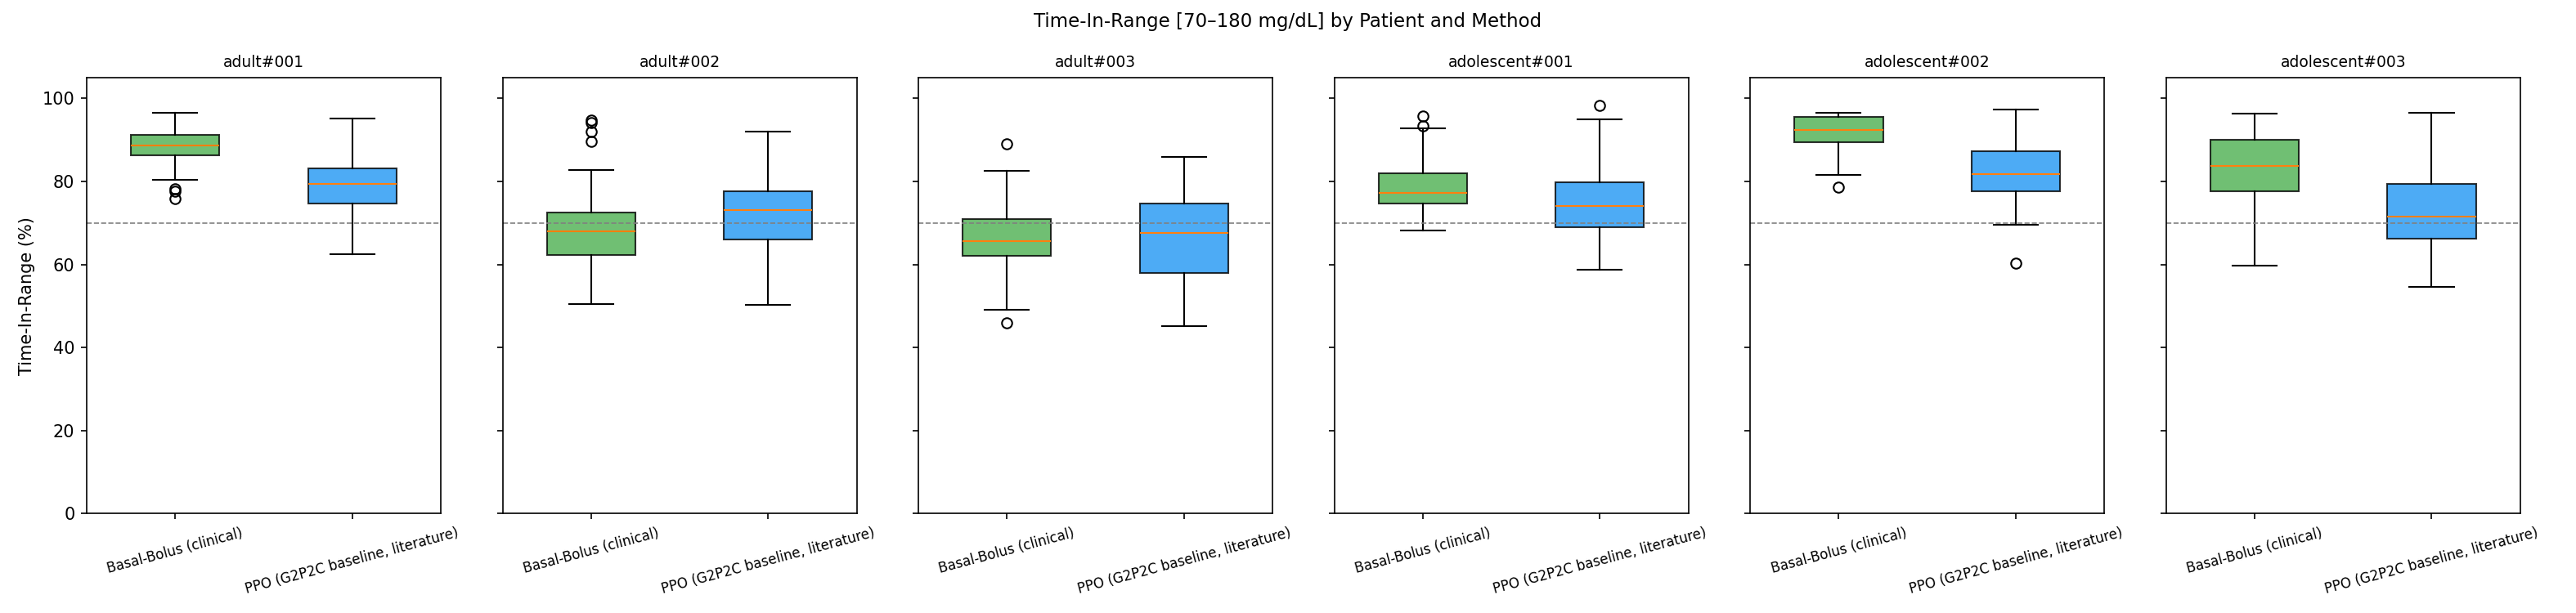
\includegraphics[width=\textwidth]{../results/figures/tir_boxplots.png}
  \caption{Distribution du TIR (\%) sur 50 épisodes par patient et par méthode. La ligne pointillée indique le seuil clinique recommandé de 70\%.}
  \label{fig:tir}
\end{figure}

\section{Taux d'échec}

Le taux d'échec (proportion d'épisodes où la glycémie franchit les seuils absolus de sécurité : $< 40$ ou $> 600$ mg/dL) constitue l'un des résultats les plus marquants de cette étude, illustré en figure~\ref{fig:failure}.

\begin{figure}[H]
  \centering
  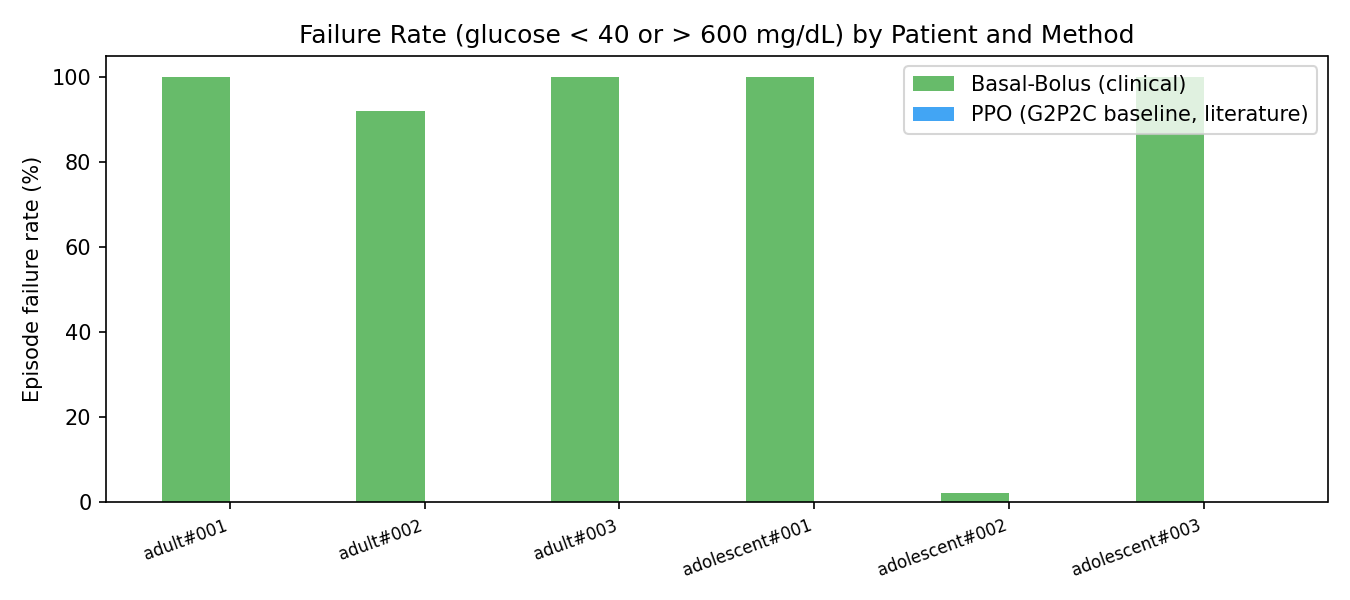
\includegraphics[width=0.85\textwidth]{../results/figures/failure_rate.png}
  \caption{Taux d'échec par patient et par méthode. Un épisode est considéré comme un échec si la glycémie sort des limites absolues de sécurité ($< 40$ ou $> 600$ mg/dL) au moins une fois.}
  \label{fig:failure}
\end{figure}

Le contrôleur Basal-Bolus présente un taux d'échec de \textbf{100\%} pour 4 des 6 patients (adultes 1, 3 et adolescents 1, 3) et de 92\% pour l'adulte 2. Seul l'adolescent\#002 est préservé (2\%). À l'inverse, l'agent PPO maintient un taux d'échec de \textbf{0\%} sur l'ensemble des patients et épisodes.

\section{Trajectoires glycémiques sur 24 heures}

Les figures \ref{fig:traj_adult001} et \ref{fig:traj_adult002} illustrent des trajectoires représentatives pour deux profils adultes. On y observe clairement les pics post-prandiaux après chaque repas (08h00, 13h00, 20h00) ainsi que la tendance du Basal-Bolus à provoquer des excursions hypoglycémiques inter-repas, tandis que l'agent PPO maintient une glycémie plus stable, légèrement plus haute en dehors des repas.

\begin{figure}[H]
  \centering
  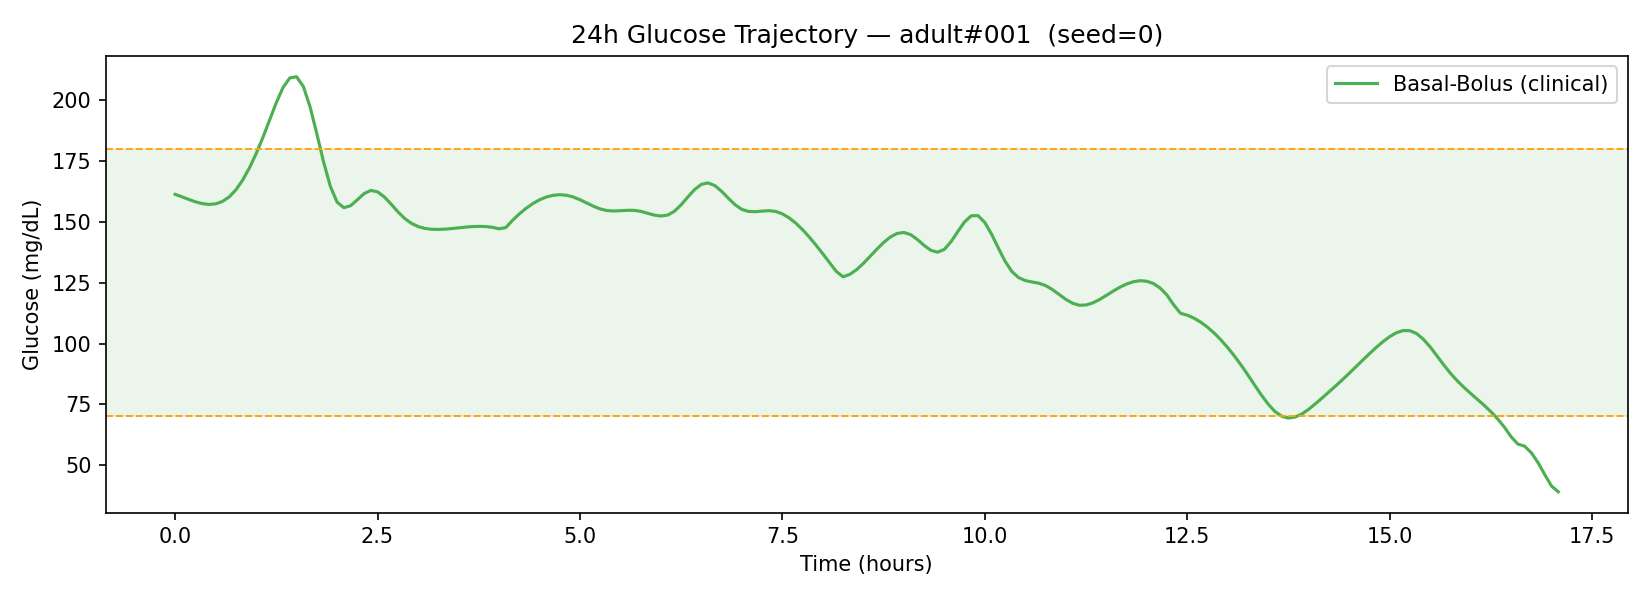
\includegraphics[width=\textwidth]{../results/figures/trajectory_adult001.png}
  \caption{Trajectoire glycémique 24h --- adult\#001, épisode de référence (graine 0).}
  \label{fig:traj_adult001}
\end{figure}

\begin{figure}[H]
  \centering
  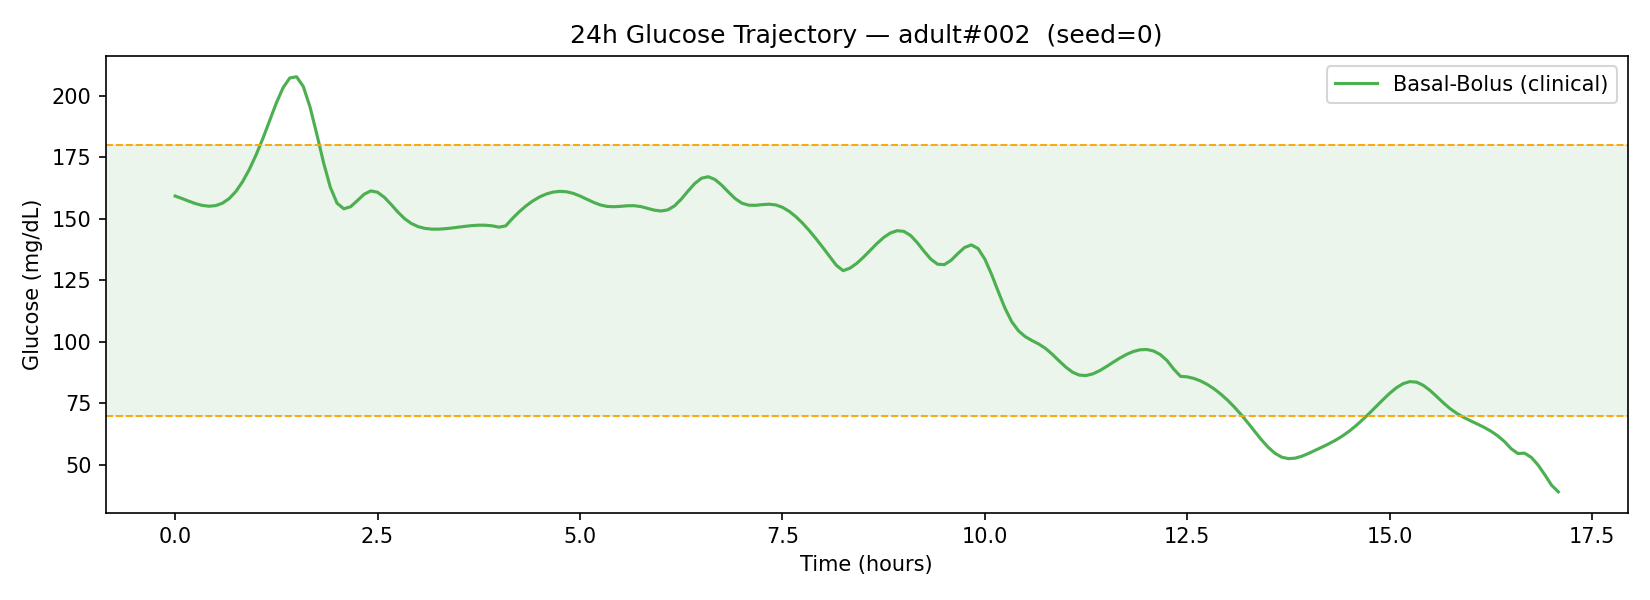
\includegraphics[width=\textwidth]{../results/figures/trajectory_adult002.png}
  \caption{Trajectoire glycémique 24h --- adult\#002, épisode de référence (graine 0).}
  \label{fig:traj_adult002}
\end{figure}

\section{Tableau comparatif des métriques par patient}

Le tableau~\ref{tab:per_patient} présente les médianes de chaque métrique clinique sur 50 épisodes, par patient et par méthode.

\begin{table}[H]
\centering
\caption{Médianes des métriques cliniques par patient (50 épisodes). En gras : meilleure valeur sur chaque ligne.}
\label{tab:per_patient}
\small
\begin{tabular}{llccccccc}
\toprule
\textbf{Patient} & \textbf{Méthode} & \textbf{TIR (\%)} & \textbf{TBR (\%)} & \textbf{TAR (\%)} & \textbf{LBGI} & \textbf{HBGI} & \textbf{Moy.} & \textbf{CV (\%)} \\
\midrule
\multirow{2}{*}{adult\#001}
  & BB  & \textbf{88.74} & 11.26 & \textbf{0.00} & \textbf{2.82} & \textbf{1.12} & \textbf{117.4} & \textbf{27.73} \\
  & PPO & 79.39 & \textbf{3.12} & 16.79 & 2.40 & 5.36 & 145.8 & 29.85 \\
\midrule
\multirow{2}{*}{adult\#002}
  & BB  & 67.90 & 32.10 & \textbf{0.00} & 6.12 & \textbf{0.92} & \textbf{103.8} & 37.74 \\
  & PPO & \textbf{73.08} & \textbf{7.38} & 21.30 & \textbf{3.32} & 6.76 & 149.0 & \textbf{30.69} \\
\midrule
\multirow{2}{*}{adult\#003}
  & BB  & 65.56 & \textbf{8.03} & \textbf{24.32} & \textbf{1.90} & \textbf{4.70} & \textbf{150.6} & \textbf{27.19} \\
  & PPO & \textbf{67.65} & 10.13 & 22.71 & 3.52 & 8.80 & 160.6 & 34.16 \\
\midrule
\multirow{2}{*}{adolescent\#001}
  & BB  & \textbf{77.22} & 21.08 & \textbf{0.00} & 4.08 & \textbf{2.09} & \textbf{122.8} & 34.14 \\
  & PPO & 73.99 & \textbf{6.01} & 19.97 & \textbf{2.77} & 7.62 & 152.4 & \textbf{31.95} \\
\midrule
\multirow{2}{*}{adolescent\#002}
  & BB  & \textbf{92.39} & \textbf{0.00} & \textbf{7.09} & \textbf{0.29} & \textbf{2.94} & \textbf{139.7} & \textbf{22.68} \\
  & PPO & 81.73 & 2.96 & 15.56 & 1.62 & 5.65 & 135.6 & 24.12 \\
\midrule
\multirow{2}{*}{adolescent\#003}
  & BB  & \textbf{83.79} & \textbf{7.91} & \textbf{8.56} & \textbf{1.82} & \textbf{3.65} & \textbf{145.2} & \textbf{24.01} \\
  & PPO & 71.49 & 7.14 & 17.68 & 2.48 & 6.92 & 149.7 & 30.33 \\
\bottomrule
\end{tabular}
\end{table}

\section{Comparaison statistique globale}

Le tableau~\ref{tab:stats} agrège les résultats sur l'ensemble des patients et présente les tests de Mann-Whitney U avec l'effet de Cohen~$r$.

\begin{table}[H]
\centering
\caption{Comparaison statistique BB vs PPO (agrégée sur les 6 patients, 300 épisodes par méthode). $p < 0.05$ : différence significative ; $r \geq 0.3$ : effet modéré.}
\label{tab:stats}
\begin{tabular}{lccccc}
\toprule
\textbf{Métrique} & \textbf{BB (médiane)} & \textbf{PPO (médiane)} & \textbf{Meilleur} & \textbf{$p$-value} & \textbf{Cohen $r$} \\
\midrule
TIR (\%)      & \textbf{80.87} & 74.81 & BB  & $<$0.001 & 0.231 \\
TBR (\%)      & 9.83  & \textbf{5.72}  & PPO & $<$0.001 & 0.336 \\
TAR (\%)      & \textbf{2.93}  & 19.27 & BB  & $<$0.001 & 0.574 \\
LBGI          & \textbf{2.40}  & 2.59  & BB  & 0.447    & 0.031 \\
HBGI          & \textbf{2.70}  & 6.75  & BB  & $<$0.001 & 0.687 \\
Moyenne (mg/dL) & \textbf{134.6} & 147.9 & BB  & $<$0.001 & 0.431 \\
CV (\%)       & \textbf{27.60} & 29.80 & BB  & 0.060    & 0.077 \\
Taux d'échec (\%) & 82.3  & \textbf{0.0} & PPO & ---      & ---   \\
\bottomrule
\end{tabular}
\end{table}

\textbf{Lecture des résultats :} sur les métriques de performance brute (TIR, TAR, HBGI, glycémie moyenne), le Basal-Bolus est statistiquement supérieur avec des effets modérés à forts. En revanche, l'agent PPO réduit significativement le TBR (effet modéré, $r=0.336$), et surtout affiche un taux d'échec nul, là où le Basal-Bolus provoque des hypoglycémies sévères ($< 40$ mg/dL) dans 82.3\% des épisodes. Le LBGI et le CV ne présentent pas de différence significative entre les deux méthodes.

\newpage

% ════════════════════════════════════════════════════════════════════════════
\chapter{Discussion}

\section{Avantages et limites du contrôleur Basal-Bolus}

\textbf{Avantages :}
\begin{itemize}
  \item \textbf{Interprétabilité} : chaque paramètre a une signification clinique directe (CIR, FSI, débit basal).
  \item \textbf{Bon TIR moyen} : sur 4 des 6 patients, le TIR médian dépasse 77\%, avec un pic à 92\% pour l'adolescent\#002.
  \item \textbf{Contrôle de l'hyperglycémie} : le TAR reste très bas (médiane 2.93\%) grâce à l'accès aux annonces de repas.
  \item \textbf{Faible HBGI} : le risque lié à l'hyperglycémie reste contrôlé (médiane 2.70).
\end{itemize}

\textbf{Limites observées :}
\begin{itemize}
  \item \textbf{Hypoglycémie systématique} : le taux d'échec de 82.3\% révèle que les formules CIR et FSI dérivées de la DTJ tendent à surestimer les besoins en insuline pour la majorité des patients virtuels, conduisant à des épisodes hypoglycémiques sévères (glycémie $< 40$ mg/dL).
  \item \textbf{TBR élevé} : avec une médiane de 9.83\%, le Basal-Bolus maintient la glycémie trop bas entre les repas pour plusieurs profils (adult\#002 : TBR médian 32\%).
  \item \textbf{Paramétrisation rigide} : les formules empiriques ne s'adaptent pas aux variations intra-individuelles au cours des 50 épisodes.
  \item \textbf{Charge cognitive} : exige que le patient estime et déclare ses glucides avant chaque repas --- contrainte éliminée par le RL.
\end{itemize}

\section{Avantages et limites de l'agent PPO}

\textbf{Avantages :}
\begin{itemize}
  \item \textbf{Sécurité absolue} : taux d'échec de 0\% sur l'ensemble des patients et épisodes. L'agent n'a jamais provoqué de glycémie $< 40$ ou $> 600$ mg/dL.
  \item \textbf{Meilleur TBR} : médiane de 5.72\% contre 9.83\% pour le BB, différence statistiquement significative ($p < 0.001$, $r = 0.336$).
  \item \textbf{Autonomie} : aucune déclaration de repas requise. L'agent infère les événements alimentaires à partir des variations de glycémie et de l'encodage temporel.
  \item \textbf{Supériorité sur adult\#002} : pour ce patient difficile (TBR BB de 32\%), le PPO obtient un TIR de 73\% contre 68\% pour le BB, tout en réduisant le TBR à 7\%.
\end{itemize}

\textbf{Limites observées :}
\begin{itemize}
  \item \textbf{TIR inférieur} : médiane de 74.81\% contre 80.87\% pour le BB, soit un écart de 6 points de pourcentage ($p < 0.001$).
  \item \textbf{Hyperglycémie post-prandiale} : sans accès aux annonces de repas, l'agent réagit aux pics glycémiques plutôt que de les prévenir, conduisant à un TAR de 19.27\% (médiane).
  \item \textbf{HBGI plus élevé} : 6.75 contre 2.70 pour le BB, indiquant un risque accru lié à l'hyperglycémie ($p < 0.001$, $r = 0.687$ --- effet fort).
  \item \textbf{Boîte noire} : la politique apprise est difficile à interpréter cliniquement, limitant la confiance des praticiens.
\end{itemize}

\section{Analyse de l'asymétrie d'information}

L'enjeu central de l'étude est l'\textbf{asymétrie d'information} délibérée entre les deux contrôleurs. Le Basal-Bolus reçoit \texttt{meal\_carbs} à chaque repas, lui permettant de calculer un bolus anticipé. L'agent PPO n'a accès qu'au triplet $[\text{glucose},\, \sin(\omega t),\, \cos(\omega t)]$.

Les résultats montrent que cette asymétrie se traduit directement sur le TAR ($+16.3$ points pour PPO) et le HBGI ($+4.05$ pour PPO) : sans annonce de repas, l'agent ne peut qu'atténuer les pics post-prandiaux, jamais les prévenir totalement. En revanche, \textbf{l'agent compense cette lacune informationnelle sur la sécurité} : ne sachant pas qu'un repas arrive, il adopte un débit basal plus conservateur, ce qui explique le TBR inférieur et l'absence totale d'épisodes catastrophiques.

Ce comportement \textit{meal-anticipating} --- visible dans les trajectoires de la figure~\ref{fig:traj_adult001} --- est une propriété émergente de la politique apprise : l'agent associe les heures typiques de repas (encodées via $\sin/\cos$) à une augmentation modérée de l'insuline, sans jamais risquer l'overdose.

\section{Implications cliniques}

Les résultats soulèvent une question fondamentale pour la certification des dispositifs médicaux : \textbf{faut-il optimiser le TIR ou éliminer les épisodes catastrophiques ?} Les deux objectifs sont en tension.

Le Basal-Bolus, malgré un meilleur TIR moyen, provoque des hypoglycémies sévères dans 82\% des épisodes --- un résultat cliniquement inacceptable qui reflète la difficulté du paramétrage individuel des formules empiriques. L'agent PPO, au contraire, n'atteint jamais les seuils critiques, ce qui est cohérent avec la fonction de récompense utilisée lors de l'entraînement (pénalité de $-100$ pour glycémie $< 40$ ou $> 600$).

Pour un déploiement en conditions réelles, un \textbf{système hybride} --- PPO pour la politique de fond, avec un module de sécurité Basal-Bolus en override lors des repas annoncés --- représenterait une piste prometteuse. Les dispositifs commerciaux actuels (Medtronic 780G, Tandem Control-IQ) intègrent d'ailleurs des approches hybrides similaires.

\newpage

% ════════════════════════════════════════════════════════════════════════════
\chapter{Conclusion et Perspectives}

Ce projet implémente un banc d'essai rigoureux pour la comparaison entre contrôle clinique classique (Basal-Bolus) et apprentissage par renforcement (PPO) dans le contexte du dosage automatique d'insuline pour le T1D. Les principaux apports sont :

\begin{enumerate}
  \item Un environnement Gymnasium complet autour du simulateur physiologique SimGlucose.
  \item Un contrôleur Basal-Bolus paramétré par patient selon les formules cliniques de référence.
  \item Un pipeline d'entraînement et d'évaluation reproductible sur 6 patients et 50 épisodes.
  \item Une batterie de métriques cliniques standardisées avec tests statistiques non-paramétriques.
\end{enumerate}

\textbf{Réponse à la question centrale :} l'agent PPO n'égale pas le Basal-Bolus sur le TIR (74.81\% vs 80.87\%, $p < 0.001$), mais il le surpasse sur la sécurité absolue (taux d'échec 0\% vs 82.3\%) et sur l'hypoglycémie modérée (TBR 5.72\% vs 9.83\%). Le résultat est nuancé : aucune méthode ne domine l'autre sur tous les critères, ce qui reflète la complexité inhérente au problème du contrôle glycémique automatisé.

\textbf{Perspectives d'amélioration :}

\begin{itemize}
  \item \textbf{Safe RL} : intégrer des contraintes de sécurité (barrières de Lyapunov, CMDP) pour garantir $\text{TBR} < 4\%$.
  \item \textbf{Méta-apprentissage} : entraîner un agent unique capable de s'adapter rapidement à un nouveau patient (MAML, Reptile).
  \item \textbf{Contrôleur hybride} : combiner un contrôleur Basal-Bolus pour la sécurité de base avec une politique RL pour l'optimisation fine, comme dans les approches \textit{shielded RL}.
  \item \textbf{Repas aléatoires} : remplacer le protocole fixe par des horaires stochastiques pour tester la robustesse à des scénarios plus réalistes.
  \item \textbf{Validation croisée} : évaluer la généralisation inter-patient (entraînement sur un sous-ensemble, test sur les patients restants).
  \item \textbf{Algorithmes avancés} : reproduire les améliorations apportées par G2P2C (apprentissage du modèle de glucose + phase de planning) sur notre infrastructure.
  \item \textbf{Validation sur données réelles} : tester la politique apprise sur le dataset OhioT1DM (12 patients réels).
\end{itemize}

\vspace{1cm}

\begin{tcolorbox}[colback=primary!5, colframe=primary, title={\color{white}\textbf{Conclusion générale}}]
La question centrale --- \emph{un agent RL peut-il égaler un contrôleur clinique de référence sans bénéficier des annonces de repas ?} --- reçoit ici une réponse quantifiée : \textbf{partiellement}. Le PPO ne rivalise pas sur le TIR global, mais offre une sécurité opérationnelle que le Basal-Bolus, tel que paramétré, ne garantit pas. Ce résultat plaide pour des approches hybrides ou pour l'intégration de contraintes de sécurité explicites (Safe RL) dans les futurs systèmes de pancréas artificiel en boucle fermée.
\end{tcolorbox}

\newpage

% ════════════════════════════════════════════════════════════════════════════
\chapter*{Références}
\addcontentsline{toc}{chapter}{Références}

\begin{enumerate}[label={[\arabic*]}]
  \item Hettiarachchi, C., Malagutti, N., Nolan, C. J., Suominen, H., \& Daskalaki, E. (2024). \textit{G2P2C --- A modular reinforcement learning algorithm for glucose control by glucose prediction and planning in Type 1 Diabetes}. Biomedical Signal Processing and Control, 90, 105839.
  \item Fox, I., Lee, J., Pop-Busui, R., \& Wiens, J. (2020). \textit{Deep Reinforcement Learning for Closed-Loop Blood Glucose Control}. Machine Learning for Healthcare Conference (MLHC), PMLR.
  \item Schulman, J., Wolski, F., Dhariwal, P., Radford, A., \& Klimov, O. (2017). \textit{Proximal Policy Optimization Algorithms}. arXiv:1707.06347.
  \item Magni, L., et al. (2011). \textit{Evaluation of a Novel Risk Measure for Type 1 Diabetes}. Journal of Diabetes Science and Technology, 5(2), 271--279.
  \item Man, C. D., Micheletto, F., Lv, D., Breton, M., Kovatchev, B., \& Cobelli, C. (2014). \textit{The UVA/PADOVA Type 1 Diabetes Simulator: New Features}. Journal of Diabetes Science and Technology, 8(1), 26--34.
  \item Cobelli, C., Renard, E., \& Kovatchev, B. (2011). \textit{Artificial pancreas: past, present, future}. Diabetes, 60(11), 2672--2682.
  \item Battelino, T., et al. (2019). \textit{Clinical Targets for Continuous Glucose Monitoring Data Interpretation: Recommendations from the International Consensus on Time in Range}. Diabetes Care, 42(8), 1593--1603.
  \item Marling, C., \& Bunescu, R. (2020). \textit{The OhioT1DM Dataset for Blood Glucose Level Prediction: Update 2020}. KDH Workshop, ECAI.
  \item Raffin, A., et al. (2021). \textit{Stable-Baselines3: Reliable Reinforcement Learning Implementations}. JMLR, 22(268), 1--8.
  \item Xie, J. (2018). Simglucose. \url{https://github.com/jxx123/simglucose}.
  \item Brockman, G., et al. (2016). \textit{OpenAI Gym}. arXiv:1606.01540.
\end{enumerate}

\end{document}